\section{Methode}\label{cha:method}

In diesem Kapitel wird die Spezialisierung eines \textit{CNN}s auf die Erkennung von Pilzbildern behandelt (siehe Kapitel \ref{cha:intr:aim}). Vorerst wird auf den Datenbeschaffungsprozess sowie der Datenvorverarbeitung eingegangen. Die darauf folgenden Abschnitte behandeln den Optimierungsprozess der \textit{Meta-Parameter} (siehe Kapitel \ref{cha:theo:backprop}, \ref{cha:theo:cnn} \& \ref{cha:theo:mod}) und erwähnen kurz diejenigen Massnahmen, welche zu einer signifikanten Verbesserung der Leistung des Erkennungsalgorithmus führten.

\subsection{Datenbeschaffung} \label{cha:met:datagathering}
Trainingsdaten bilden die Grundlage jedes auf \textit{Machine Learning} basierenden Algorithmus, weswegen man ein solides Fundament aus vielen Trainingsdaten benötigt (siehe Kapitel \ref{cha:theo:ml:training}). Da die Datenlage für Pilzbilder hingegen eher schlecht ist, ist die Datenbeschaffung ein wichtiger Bestandteil dieser Arbeit. Dabei gilt es, möglichst viele korrekt bestimmte Pilzbilder zu sammeln.

Für das Training sollen von jeder der 20 ausgewählten Pilzarten (siehe Tabelle \ref{table:shrooms}) mindestens 230 verschiedene Bilder beschaffen werden, von den unbekannten 1840 (das Achtfache). Um die Leistung des Algorithmus mittels unabhängigen Daten zu testen (siehe \textit{Validierung} in Kapitel \ref{cha:theo:ml:b-v}), werden zusätzlich 20 Bilder pro bekannte Art resp. 160 für die unbekannte Kategorie gesammelt. Somit mussten 250 Bilder pro ausgewählte Art sowie 2000 Bilder von unbekannten Arten gesammelt werden, insgesamt also etwa 7000 Bilder. Die Anzahl der bekannten Arten begründet sich mit den schwer verfügbaren Bilddaten, die der unbekannten durch eine erfahrungsgestützte Abschätzung, um im Rahmen einer Maturarbeit zu bleiben und trotzdem noch aussagekräftige Ergebnisse erhalten zu können.

Folgende Massnahmen wurden ergriffen, um möglichst viele, reine Trainingsdaten zu beschaffen:

\subsubsection{Datenbank SwissFungi}
Um einen Grunddatensatz zu erhalten, wurde die Fotodatenbank vom offiziellen SwissFungi Pilzatlas der WSL Schweiz verwendet\cite{wsl}. Von den 20 ausgewählten Arten konnten dadurch je einige Dutzend Bilder gesammelt werden; von den unbekannten Arten konnte die geforderte Anzahl von 2000 Exemplaren gedeckt werden. Diese Bilder sind alle professionell bestimmt und bedürfen daher keiner weiteren Kontrolle um die Datenreinheit zu garantieren. 

\subsubsection{Webseite ShroomNET}
Um Pilzsammler und Pilzfotografen aus der Region einfach zu erreichen, wurde die Webseite \textit{www.obermeier.ch} mit einem Hochladeformular für Pilzbilder eingerichtet. Aus einer Liste der ausgewählten Arten lässt sich die Kategorie auswählen, wobei die hochzuladenden Bilder mittels Drag-and-Drop direkt hochgeladen werden. Neben der Hochladefunktion wurde um die Datenreinheit zu gewährleisten zusätzlich ein \textit{Quiz} erstellt, bei dem Besucher die hochgeladenen Pilzbilder klassifizieren können. Mithilfe dieser Webseite lassen sich somit einfach weitere Bilder zusammentragen, welche auch direkt von erfahrenen Sammlern verifiziert werden können (siehe Abbildung \ref{img:webpage}).

Verbreitet wurde die Webseite über Telefonate und Mail-Verkehr mit Pilzkontrolleuren aus der Region Brugg-Aarau sowie in einem Artikel der Schweizerischen Zeitschrift für Pilzkunde SZP\cite{szp}, welche in der ganzen Schweiz versendet wurde. Mittels der Webseite konnten nochmals insgesamt etwa 300 Bilder gesammelt werden.

\subsubsection{Internet Crawler}
Mithilfe eines Python-Skriptes\cite{crawler} konnten automatisiert mit der Google-Suchmaschine nochmals etwa 400 Bilder pro Art gefunden und heruntergeladen werden, gesucht wurde dabei nach dem wissenschaftlichen Namen der Pilze. Aufgrund vieler Unreinheiten waren pro Kategorie nur etwa 150 weitere Bilder brauchbar. Da die Google-Suche nicht immer korrekte Ergebnisse liefert, wurden diese Bilder auf die Webseite hochgeladen, um sie im \textit{Quiz} nochmals von Pilzsammlern verifizieren zu lassen. 

\subsubsection{Videos}
Eine weitere Möglichkeit, um an viele Bilddaten zu kommen, ist das Extrahieren von Standbildern aus Videos. Bei sich ändernden Kameraperspektive lassen sich mehrere Standbilder von selben Pilz anfertigen, welche nicht identisch sind und sich daher als Trainingsdaten eignen. Dafür wurde das von Michael Bachmeier\cite{bachmeier} zur Verfügung gestellte Videomaterial verwendet. Insgesamt liessen sich durch die Bearbeitung von Videos weitere 1500 Bilder zur Datenbank hinzufügen. Auch diese Daten bedürfen aufgrund der zuverlässigen Quelle keiner weiteren Kontrolle.

\subsection{Datenaufbereitung} \label{cha:met:preprocessing}
Nach dem Sammeln der rohen Bilddaten gilt es in der Aufbereitung darum, die Bilder auf das Training anzupassen, d.h. Zentrieren sowie bildfüllendes Skalieren des Pilzes\footnote{Zwar könnten die Daten auch unbearbeitet in das Training eingespeist werden, jedoch erschwert die zusätzliche Lokalisierung des Pilzes den Lernprozess und führt unweigerlich zu einer Verschlechterung der Erkennungsleistung. Das Problem der Objektfindung in Bildern soll nicht Teil der Problemstellung sein, weswegen dieser Schritt hier manuell verrichtet wird.}. Dafür wurde eine Mindestauflösung von $200 \times 200$px festgelegt, welches eine gute Balance zwischen Details im Bild und Komplexität des Netzes bildet. Ein zu diesem Zwecke mit MatLab programmiertes Hilfsprogramm beschleunigte den manuellen Bearbeitungsprozess von Bildern wie auch Videos.
\begin{figure}[h]
	\centering
	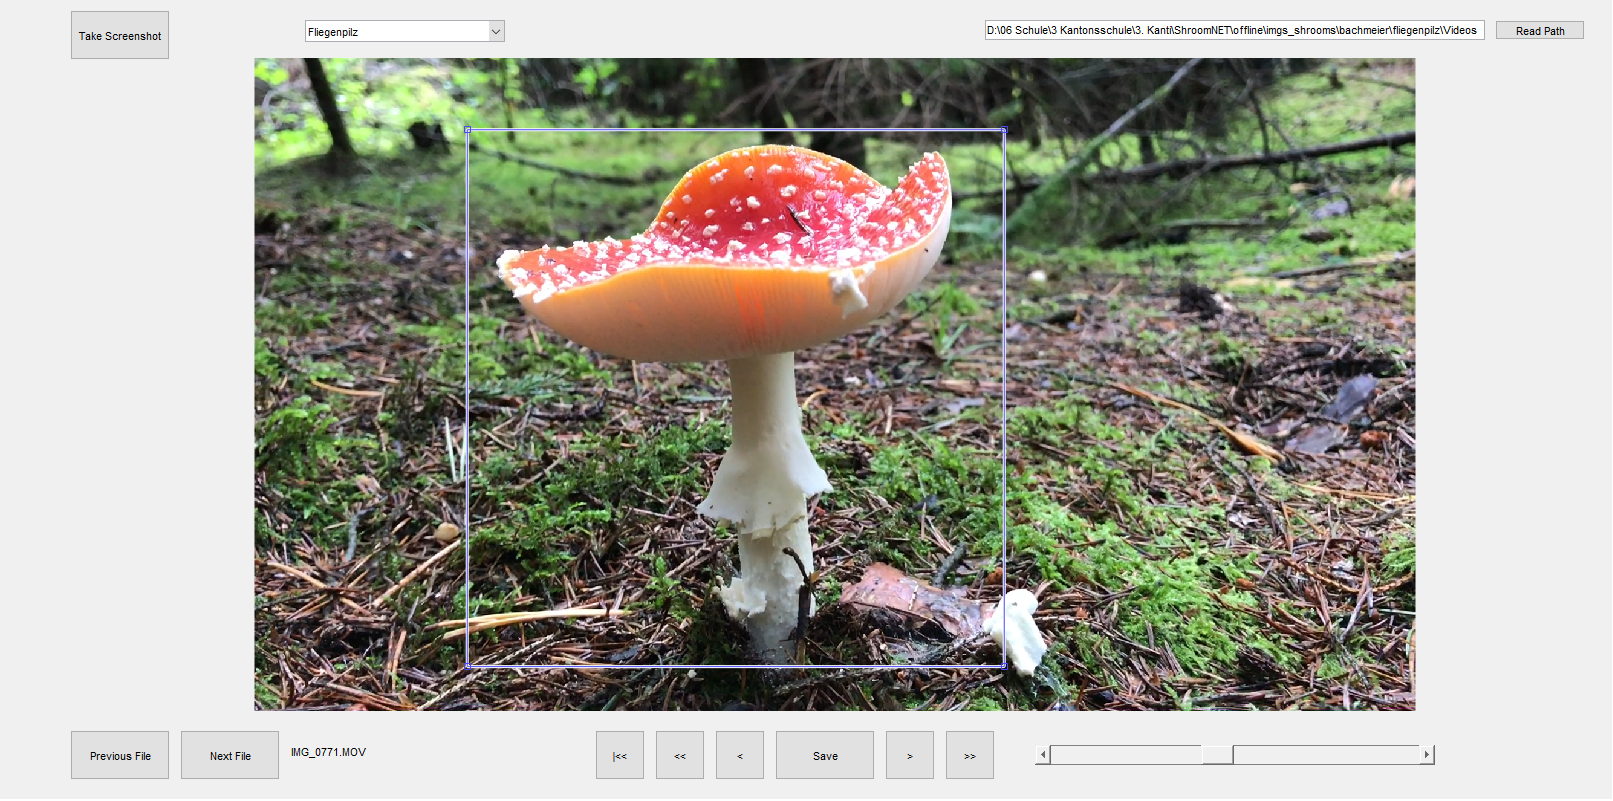
\includegraphics[width=\textwidth]{cropping}
	\caption[\textit{\textit{Hilfsprogramm}}]{Screenshot vom Hilfsprogramm beim Bearbeiten eines Videos: Oben links kann die Kategorie ausgewählt werden, der blaue Rahmen legt den Bildausschnitt fest. Unten befinden sich Steuerelemente zur Navigation sowie Speicherung des zugeschnittenen Bildes.}
	\label{img:precrocessing}
\end{figure}

Die zugeschnittenen Daten wurden in den vorher festgelegten Proportionen zufällig in Trainings- und Validierungsdaten unterteilt. Die aus Videos extrahierten Trainingsdaten eignen sich aufgrund der in Abbildung \ref{img:video_frames} ersichtlichen Ähnlichkeit nicht zur Validierung\footnote{Die Ähnlichkeit führte in ersten Tests zu einer Verfälschung der Ergebnisse.}, stattdessen werden diese ausschliesslich als Trainingsdaten verwendet.

\begin{figure}[h]
	\centering
	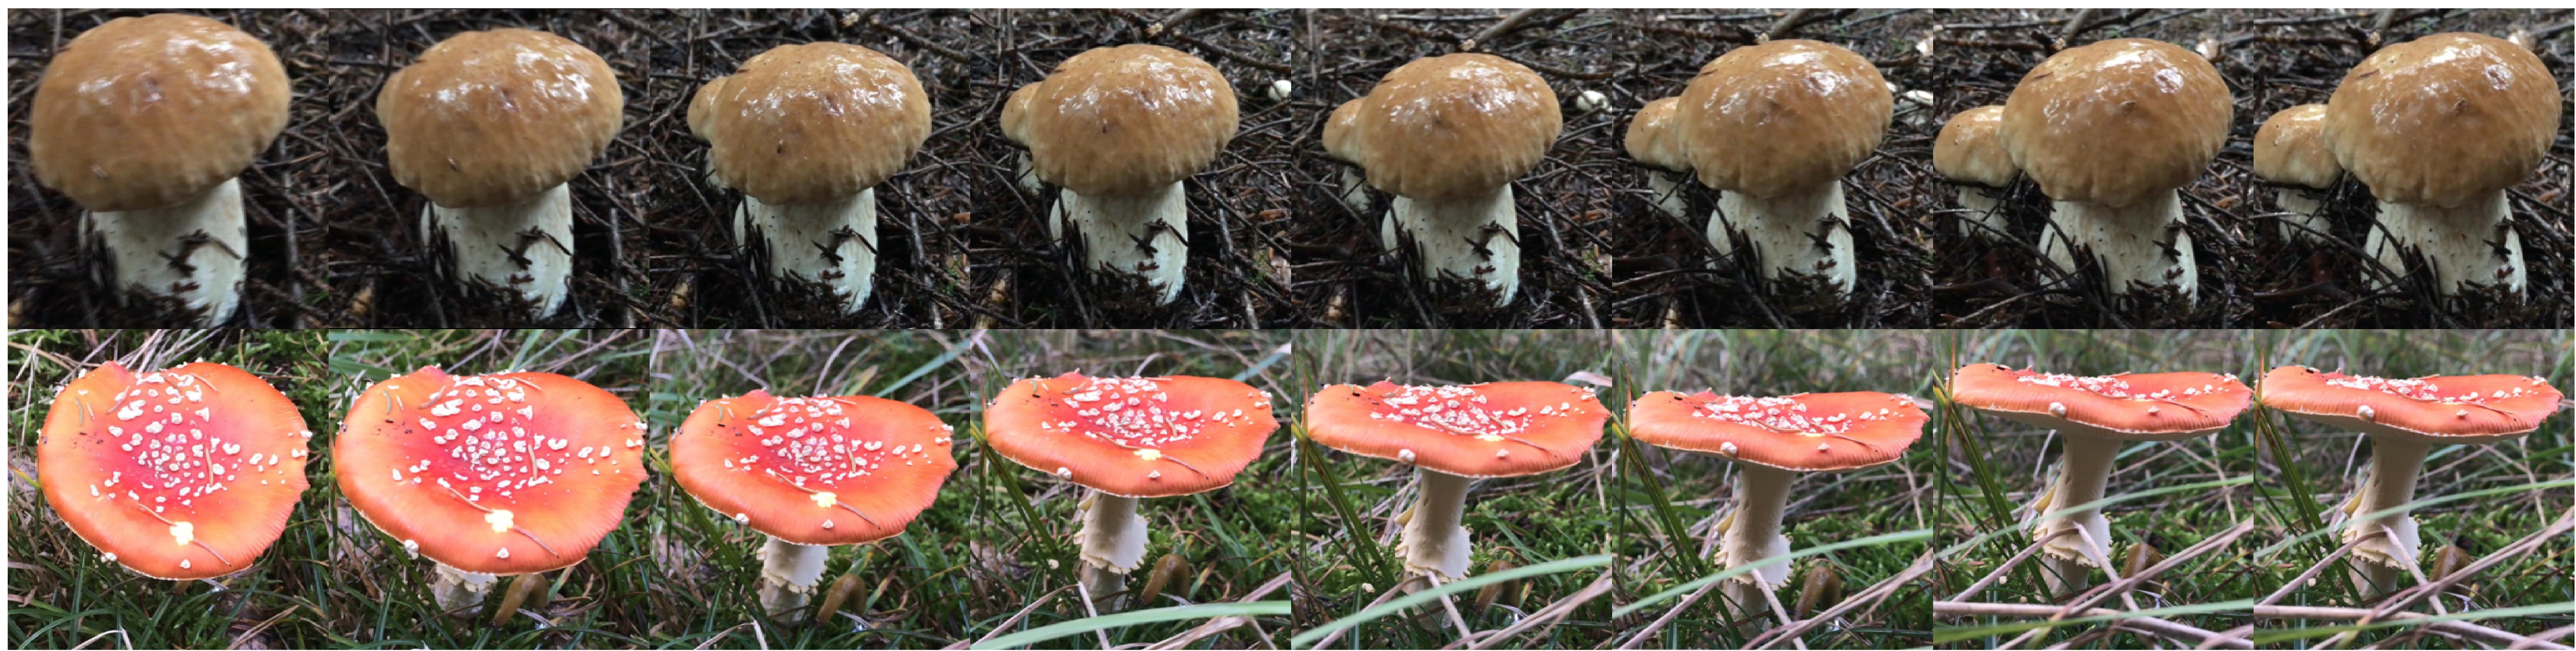
\includegraphics[width=\textwidth]{video_frames}
	\caption[\textit{\textit{Video-Frames}}]{8 Standbilder aus 2 Videos}
	\label{img:video_frames}
\end{figure}

Von gewissen Pilzarten waren weitaus mehr als 230 Bilder vorhanden. Dieser Überschuss musste ausgeglichen werden, damit von jeder Art gleich viele Trainingsbilder vorhanden sind. Statt diese überzähligen Exemplare aus dem Training auszuschliessen, wurden die Trainingsbilder mit Kopien zufälliger Exemplare der selben Kategorie auf 400 Bilder pro Pilzart ergänzt\footnote{Die Programmierumgebung von MatLab lässt keine benutzerdefinierte Verhältnisse der Kategorien zu, ohne tiefliegende Modifikationen an der \textit{Neural Network Library} vornehmen zu müssen. Daher diese Problemumgehung mittels Duplizieren einiger Trainingsdaten.}.


%Zusammengefasst ergeben sich aus der Datenbeschaffung und Datenaufbereitung folgende Zusammensetzung der Trainings- und Validierungsdaten:
%\begin{center}
%	\begin{tabular}{l | l | l | l | l}
%		Quelle & Training  & Training  & Validierung  & Validierung \\
%		  & bekannt & unbekannt & bekannt & unbekannt\\
%		\hline
%		SwissFungi & ca. 25 & 1840 & ca. 5 & 160\\
%		Webseite & ca. 15 & 0 & ca. 3 & 0\\
%		Crawler & ca. 130 & 0 & ca. 12 & 0\\
%		Video & ca. 75 & 0 & 0 & 0\\
%		\hline
%		\hline
%		& mind. 230
%	\end{tabular}
%\end{center}

\subsection{Entwicklungsprozess}\label{cha:met:dev}
Mit den aufbereiteten Trainingsdaten gilt es im nächsten Schritt den Algorithmus für die Pilzartenerkennung zu erarbeiten. In diesem Projekt wird hierfür die Entwicklungsumgebung MatLab mit der \textit{Deep Learning Toolbox}\cite{matlab} verwendet. Die Entscheidung fiel auf MatLab aufgrund des effizienten und einfach zu modifizierenden Grundgerüstes für \textit{Deep Learning} und \textit{KNN}s. Die Unterstützung von Mehrkernprozessoren sowie die Einbindung von Grafikkarten beschleunigt zudem den Trainingsprozess merklich. Auch sind in MatLab bereits vortrainierte \textit{KNN}s für das \textit{Transfer-Learning} (siehe Kapitel \ref{cha:theo:mod:tl}) einfach zu implementieren und modifizieren.

In den folgenden Schritten wird beschrieben, welche Modifikationen zu einer signifikanten Verbesserung der Bestimmungsleistung beigetragen haben. Dabei in diesem Kapitel wie auch in der Diskussion der Prozentsatz der richtig erkannten \textit{Validierungsdaten} als Metrik für den Vergleich der Algorithmen dienen.

\subsubsection{Bezugswert}
Um bestimmen zu können, ob ein Algorithmus tatsächlich aus den gegebenen Daten lernt und nicht durch Zufall die korrekte Lösung errät, gilt es im ersten Schritt einen Richtwert für die Leistung zu finden. Diesen Wert gilt es von den Algorithmen zu übertreffen. Bei 21 Klassen kann durch zufälliges Zuteilen von Antworten eine Genauigkeit von $\frac{1}{21} \approx 4.76\%$ erreicht werden. Mit den in Kapitel \ref{cha:met:preprocessing} gegebenen Klassenverhältnissen ist es jedoch viel naheliegender, jedes Bild der unbekannten Kategorie zuzuteilen. Mit dieser Strategie erhält man eine Genauigkeit von $\frac{8}{20+8} \approx$\textbf{28.6\%}. Letzterer Wert wird aufgrund der Einfachheit sowie der besseren ''Leistung'' als Bezugswert für folgende Algorithmen verwendet.

\subsubsection{Basis-SNN}
Der erste Algorithmus besteht aus einem einfachen \textit{SNN} mit einem \textit{Fully-Connected-Layer} als \textit{Hidden-Layer} und einem weiteren \textit{Fully-Connected-Layer} als \textit{Output-Layer}; die Bilder werden mittels Normalisierung gemittelt.
%Wie bereits im Kapitel \ref{cha:theo:dl} erwähnt worden ist, sollte theoretisch ein entsprechend grosser \textit{Hidden-Layer} für die korrekte Bestimmung aller Pilzbilder genügen.
Um ein grobes Bild der Leistung zu erhalten, werden folgende \textit{Meta-Parameter} des \textit{SNN}s variiert: Die Eingangsdatengrössen (200$\times$200px, 50$\times$50px oder 10$\times$10px) sowie die \textit{Hidden-Layer}-Grösse ($20$, $60$ oder $100$ Neuronen). Für die restlichen \textit{Meta-Parameter} dienen vorerst Werte, welche sich erfahrungsgemäss für ähnliche Bilderkennungsprobleme bewährt haben. Alle \textit{Meta-Parameter} sind in der Tabelle \ref{table:basic_snn_training} im Anhang zu finden. Folgend die Ergebnisse:

\begin{table}[h]
	\begin{center}
		\def\arraystretch{1.4}
		\begin{tabular}{c | c | c | c }
			& \multicolumn{3}{l}{Anzahl \textit{Hidden-Neuronen}} \\
			Bildauflösung & 20 & 60 & 100\\
			\hline
			$200\times200$px& 3.6\%& 3.6\% & 3.6\%\\
			$50\times50$px& 12.5\% & 13.6\% & 20.4\%\\
			$10\times10$px& 41.3\% & \textbf{43.6\%} & 40.2\%\\
		\end{tabular}
	\end{center}
\caption[Bestimmungsleistung von \textit{SNN}s]{Bestimmungsleistung von \textit{SNN}s im einem \textit{Hidden-Layer}}
\label{table:snn}
\end{table}

Bemerkenswert ist das Ergebnis für das \textit{SNN} mit 60 \textit{Hidden-Neuronen}, welches die kleinsten Eingangsdaten erhalten hat: Mit nur 0.25\% der vorhandenen Daten leistet es mehr als das Zehnfache wie die Netze, welche alle 200$\times$200$\times$3 (Auflösung $\times$ Farbkanäle) Datenpunkte erhalten haben, und fast das Doppelte des Bezugswertes. Der nächste Schritt ist es nun, die Komprimierung der Informationen nicht durch verlustbehaftetes Skalieren zu Erreichen, sondern durch Hinzufügen von zusätzlichen \textit{Convolution-Layers}.

\subsubsection{Basis-CNN}
Als Grundlage für das \textit{CNN}s dient ein nur aus \textit{Convolution-Layers}, \textit{Pooling-Layers} und einem \textit{Fully-Connected-Layer} (entspricht dem \textit{Output-Layer}) zusammengesetztes Netz (komplette Liste der \textit{Meta-Parameter} siehe Tabelle \ref{table:basic_cnn_training}). Als grobe Vorlage für Einstellungen der drei \textit{Convolution-Pooling-Einheiten} diente \textit{AlexNet}\cite{alexnet}. Die Auflösung der Eingangsdaten wird für das Training des \textit{CNN}s bei 200$\times$200px belassen, da die Filterung von den relevanten Informationen den \textit{Convolution-Layers} überlassen werden dann.

\begin{figure}[h]
	\centering
	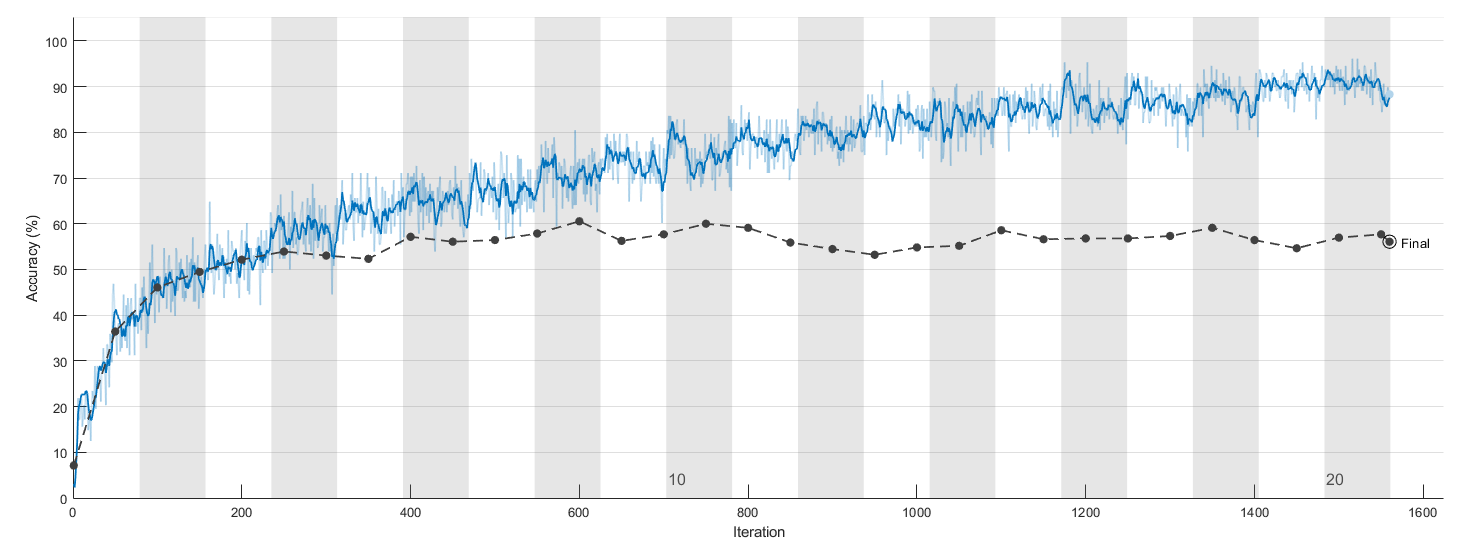
\includegraphics[width=\textwidth]{baseline_cnn}
	\caption[\textit{\textit{Trainingsverlauf Basis-\textit{CNN}}}]{Trainingsverlauf vom Basis-{CNN}: Leistung mit Trainingsdaten in blau, Leistung mit Validierungsdaten in grau}
	\label{img:baseline_cnn}
\end{figure}

Nach dem Training erreichte das \textit{Basis-CNN} mit den Trainingsdaten eine Genauigkeit von 88.3\%. Mit den Testdaten etwa ein Drittel weniger: \textbf{56.1\%}. Wie in der Abbildung \ref{img:baseline_cnn} zu erkennen ist, verbessert sich die Leistung der Trainingsdaten (blau) kontinuierlich, die der Validierungsdaten (grau) jedoch stagniert ab Epoche 8 (Iteration 600). Dies ist ein typisches Verhalten eines überangepassten Algorithmus(siehe \textit{Überanpassung} in Kapitel \ref{cha:theo:ml:b-v}). Um dem entgegenzuwirken sollen die Trainingsdaten im nächsten Abschnitt künstlich erweitert werden.


\subsubsection{Data-Augmentation} \label{cha:met:da}
Wie in Kapitel \ref{cha:theo:mod:da} beschrieben, wenden mittels dem in MatLab vorhandenen \textit{Data-Augmentation-Tool} (sog. \textit{augmentedImageDatastore}) künstlich durch Verschieben, Rotieren und Spiegeln des Bildes ''neue'' Trainingsdaten generiert. Alle Einstellungen zur \textit{Data-Augmentation} sowie \textit{Meta-Parameter} sind in der Tabelle \ref{table:dataaug_training} im Anhang zu finden.

Nur mit künstlich erweiterten Trainingsdaten erreichte das ansonsten gleiche \textit{CNN} eine Leistung von \textbf{63.4\%}. Zudem ist in Abbildung \ref{img:dataaug_cnn} auch deutlich zu erkennen, dass die Differenz zwischen Validierungsdaten und Trainingsdaten (67.2\%) massiv kleiner ist.

\begin{figure}[h]
	\centering
	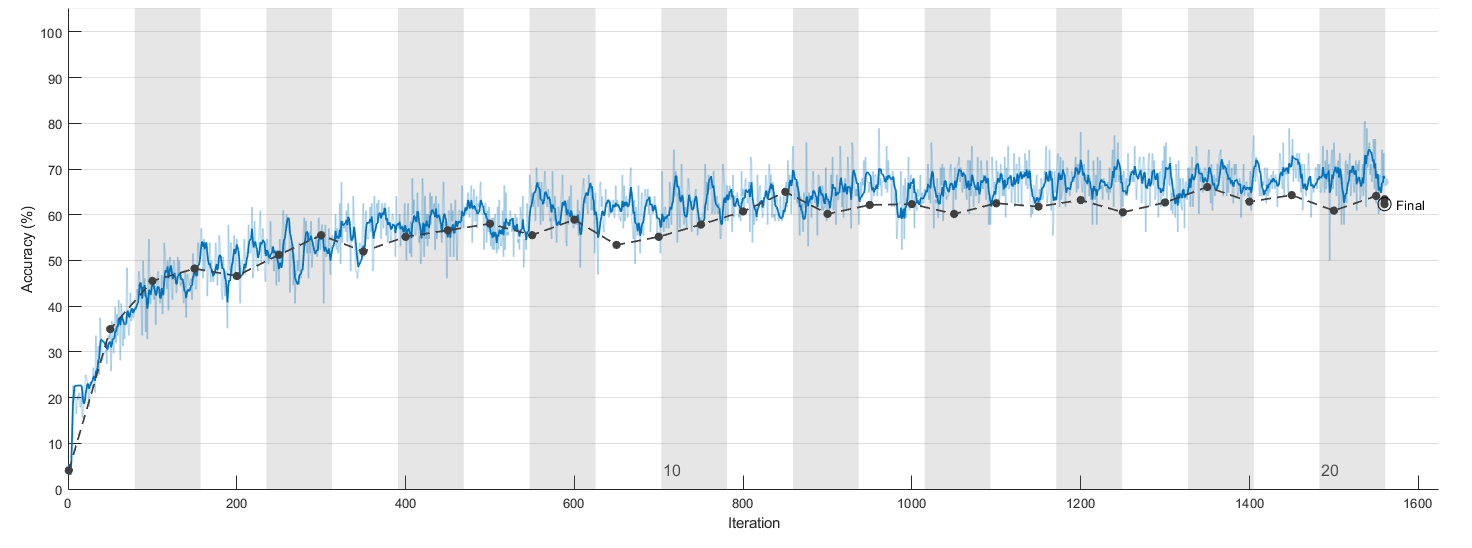
\includegraphics[width=\textwidth]{dataaug}
	\caption[Trainingsverlauf Basis-\textit{CNN} mit \textit{Data-Augmentation}]{Trainingsverlauf vom Basis-{CNN} mit \textit{Data-Augmentation}: Leistung mit Trainingsdaten in blau, Leistung mit Validierungsdaten in grau}
	\label{img:dataaug_cnn}
\end{figure}

\subsubsection{Farbfilter}
Um dem Algorithmus zusätzlich zu unterstützen, kann man durch Hinzufügen eines einfachen Farbfilters Farbbereiche löschen, welche keine relevanten Informationen tragen. Im Fall der Pilzerkennung ist Grün in grossen Mengen im Hintergrund vertreten, welches mittels eines Grün-Filters auf den für das \textit{CNN} neutralen Wert 0 (nach der Anwendung der Bild-Normalisierung) gesetzt werden kann.

Nach dem Training (Gleiche \textit{Meta-Parameter} wie \textit{CNN} aus Abschnitt \ref{cha:met:da}, siehe Tabelle \ref{table:dataaug_training} im Anhang) erreichte man ein ähnliches Resultat wie ohne Filter (60.71\%), jedoch unterschieden sich die Methoden in der Laufzeit: Das Filtern der Grün-Töne für jedes Trainingsexemplar verdoppelte fast die Berechnungszeit (45 gegenüber 27 Minuten).

\begin{figure}[h]
	\centering
	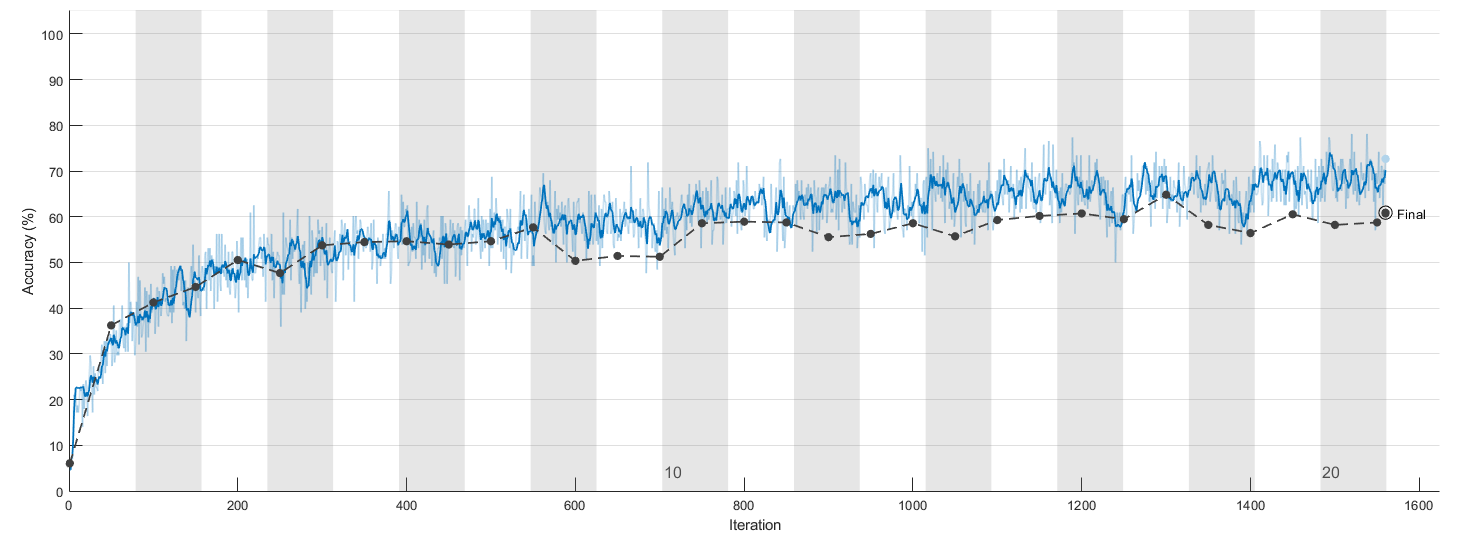
\includegraphics[width=\textwidth]{dataFilter}
	\caption[Trainingsverlauf Basis-\textit{CNN} mit Grün-Filter]{Trainingsverlauf vom Basis-{CNN} mit Grün-Filter: Leistung mit Trainingsdaten in blau, Leistung mit Validierungsdaten in grau}
	\label{img:gf_cnn}
\end{figure}

Aus dem ähnlichen Ergebnis lässt sich schliessen, dass das \textit{CNN} die für die Bestimmung relevanten Farben ohne externer Unterstützung filtern kann, was wiederum auf eine robuste Netzarchitektur deutet. Aufgrund des zusätzlichen zeitlichen Aufwands wird diese Massnahme nicht in den folgenden \textit{CNN}s implementiert.

\subsubsection{Justierung des CNNs}
Da die \textit{Meta-Parameter} des Basis-\textit{CNN}s nur durch eine erfahrungsgestützte Schätzung eingestellt worden sind, gilt es in diesem Kapitel die \textit{Meta-Parameter} zu justieren. Dabei sollen weitere \textit{Layers} und \textit{Layer-}Typen verwendet werden, um das \textit{CNN} weiter auf die Pilzartenerkennung zu spezialisieren. Da es für die Zusammenstellung sowie Einstellung von \textit{Layern} unzählige Kombinationsmöglichkeiten gibt, soll nur ein kleiner Bereich möglichst systematisch untersucht werden.

\subsubsection{Einspeisung von Zusatzinformationen}

\subsubsection{Transfer-Learning}

\subsubsection{CNN-Ensemble}